\documentclass[12pt, oneside]{article} 
\usepackage{amsmath, amsthm, amssymb, calrsfs, wasysym, verbatim, bbm, color, graphics, geometry, enumitem, array, multirow, hyperref, tabulary, xcolor}

\usepackage{amsmath,amssymb,mathtools} % do fancy math
\usepackage{graphicx} % import images
\usepackage{xcolor}
\usepackage{tikz} % draw images with latex
\usepackage{listings} % for code 
\usepackage{enumitem, bm, bbm}
% \usepackage{amsfonts}
\usepackage[onehalfspacing]{setspace}

\usepackage{subcaption}




\setlength{\parindent}{0in} % set paragraph indent
\everymath{\displaystyle}
\setlist{noitemsep}


\geometry{top=1in, bottom=1in, left=1in, right=1in}
\setlist{noitemsep}
%\setcounter{secnumdepth}{0} % comment this out for section numbering
\everymath{\displaystyle}

\geometry{top=1in, bottom=1in, left=1in, right=1in}
\setlist{noitemsep}
%\setcounter{secnumdepth}{0} % comment this out for section numbering
\everymath{\displaystyle}

\newcommand*{\IC}{\mathbb{C}}
\newcommand*{\IR}{\mathbb{R}}
\newcommand*{\DFT}{\operatorname{DFT}}


\title{Finance}
\author{Boomer}
\date{December 2020}


\linespread{1.3}
\begin{document}

\maketitle

\newpage

\tableofcontents

\newpage

\section{Using Dark Pool Short Sales as a Proxy for Buying Activity}

  According to the SEC, trades marked with the seller "short" comprise 49\% of equity share volume. In other words, half of all selling volume in market is short selling. (This cannot be all speculative short selling)


\subsection{Short Sales}
    \begin{itemize}
         \item Traditionally, Market makers (MM's) make their money by "quoting a spread".
         \item Ex: Placing bid at \$19.95 and offer at \$20.00. 
         \\Since MM has not position in the stock, the offer at \$20.00 is a short sale.
         \item Suppose one investor \textit{sells} to MM at \$19.95 and another \textit{buys} from MM at \$20.00. \\Then only the trade where the investor is buying stock at \$20.00 is reported as "short".
         \item \textbf{Thus:} Short volume = investor buying volume, Non-short volume = investor selling volume.
         No coincidence that short volume is predictably \textit{half} of total volume (buying half of the market).
         \item Note: Speculative short sellers (tiny volume), passive sell orders from traders who aren't market makers (Trades showing up as \textit{not} short) will not throw off this number by a lot.
         \item These assertions hold due to the \textbf{rebates} a MM receives when a trader "takes" the liquidity that the MM offered at the bid or offer. HFT's is the result of the scramble for rebates.
         \item If you submit an order to buy 100 shares at market, you will buy those from an HFT MM. If you later submit a passive limit order to sell 100 shares at the offer, you will sell those shares to an HFT MM (once someone buys 100 shares from him at a higher price elsewhere). Although this is "frontrunning", the competition by MM's to garner rebate has been beneficial for the average investor (by providing liquidity).
         \item Lucky for us, the middle-man always leaves a trail - he is compelled to sell short whenever he fills a buy order.
        \begin{figure}[!ht]
            \centering
            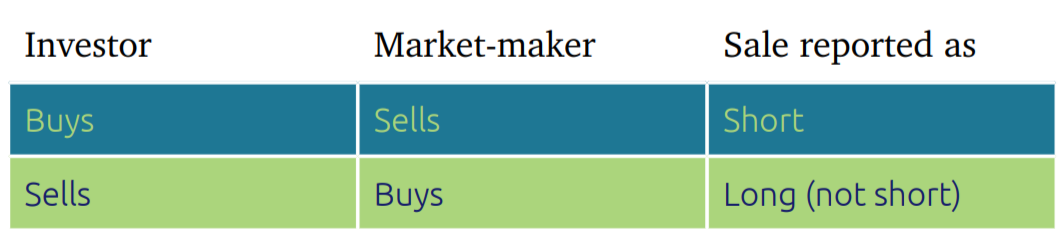
\includegraphics[width=\textwidth]{Capture.PNG}        
            %\caption{Caption}
            %\label{fig:my_label}
        \end{figure}
    \end{itemize}
\newpage
\subsection{Hypothesis: Short = Long}

\begin{itemize}
    \item H\textsubscript{0}: High short sale volume is positively correlated to intraday stock gains
    \item Since there is no real-time short sale reporting requirement, we use FINRA's short sale volume data from their Trade Reporting Facilities(TRFs). 
    \item The TRFs receive data from exclusively off-exchange or dark venues and some are internalizers.
    \item Since the analysis doesn't need to distinguish between types of off-exchange venues. all data from TRFs will be referred to as dark pool data.
    \item Benefit of dark pools: No visible order book/quoting, can buy/sell between bid and ask.
    \item For a MM in the dark pool, midpoint trades mean spreads become even tighter (sub-penny), but rebate is still king. 
    \item Only concern is that short volume data from dark pools as a proxy for the whole market is that it just isn't enough data. 
    \item Fortunately, off-exchange volume accounts for about 1/3 of all trade volume. 
\end{itemize}

\subsection{Method}
\begin{itemize}
    \item Find average intraday return (open to close) of all exchange-listed U.S. stocks, preferreds, CEFs, ETFs, ETNs, etc from 2010 to present. 
    \item This is the baseline return.
    \item Breakdown intraday returns according to the ratio of dark pool short volume to long volume on any given day. 
\end{itemize}

\subsection{Results}
\begin{itemize}
    \item Naturally, we expect to see that a higher short volume (representative of buying activity) is correlated to higher intraday returns. 
    \item Across a universe of 11,254 securities, listed between 2010 and present, the mean intraday return of this data is 0.003\% over a sample of 12.74 million discrete days of returns.
    \item When we subsequently halve the data acording to dark pool short volume composition, the lower quantile being 0-49\% short and the upper being 50-100\% short, we find that the mean intraday return of the lower quantile is -0.0593\% and the upper, 0.1184\%
\end{itemize}
 \begin{figure}[!ht]
    \centering
    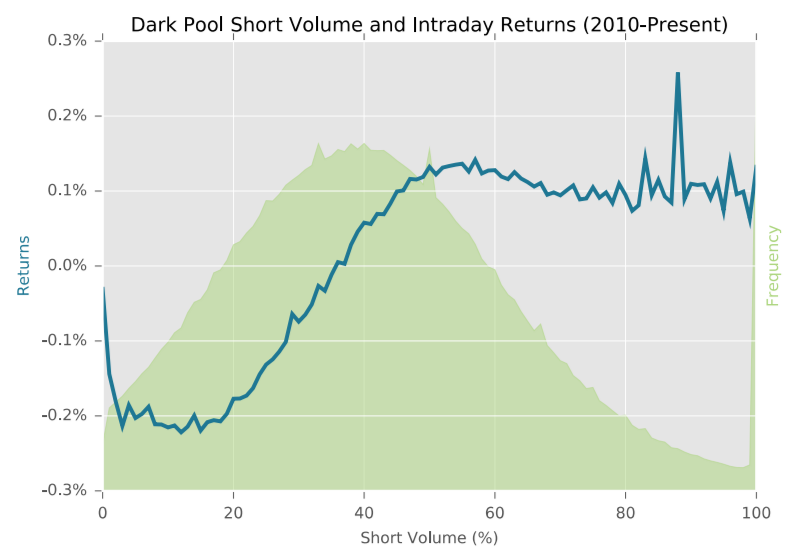
\includegraphics[width=\textwidth]{Dark Pool Short Volume and Intraday Returns (2010-Present).png}        
    %\caption{Caption}
    %\label{fig:my_label}
\end{figure}

\begin{itemize}
    \item Focusing on the part of the figure where data is most abundant(thus most relevant), there is a linear relationship between short volume and and intraday returns from 20\% to 60\%.
    \item Exceptionally low short volume will often be linked to days with large block trades between two parties with no market-making intermediary. 
    \item Exceptionally high short volume will often be linked to either large buy orders facilitated by a broker or a high volume of speculative short sales.]
    \begin{itemize}
        \item A few large block orders originating in dark pools is likely the cause of lower than average(~40\%) aggregate dark pool short volume
    \end{itemize}
    \begin{itemize}
        \item There is a high incidence of data where 100\% of volume is short. This is likely broker-dealer shorting shares into a customer account as one leg of a transaction in a very illiquid stock.
    \end{itemize}
\end{itemize}

\subsection{Extrapolation}
\begin{itemize}
    \item Dark Index (DIX) has chronicled, in dollar-weighted terms, dark pool short volume across components of the S\&P 500 since 2011. 
    \item Because the index is dollar-weighted, volume is multiplied by share value, giving more weight to larger and more frequently traded stocks. 
    \item $\geq$ 45\% of dollar weighted short volume are associated with mean 60-market-day returns of 5.3\% compared to a mean of 2.8\% across the whole data set.
    \item Since DIX tends to rise into corrections, we believe that it reflects a broad willingness of investors to accumulate S\&P 500 component stocks at lowered valuations, and that high levels of short volume correspond to positive medium-to-long term investor outlooks. 
\end{itemize}
 \begin{figure}[!ht]
    \centering
    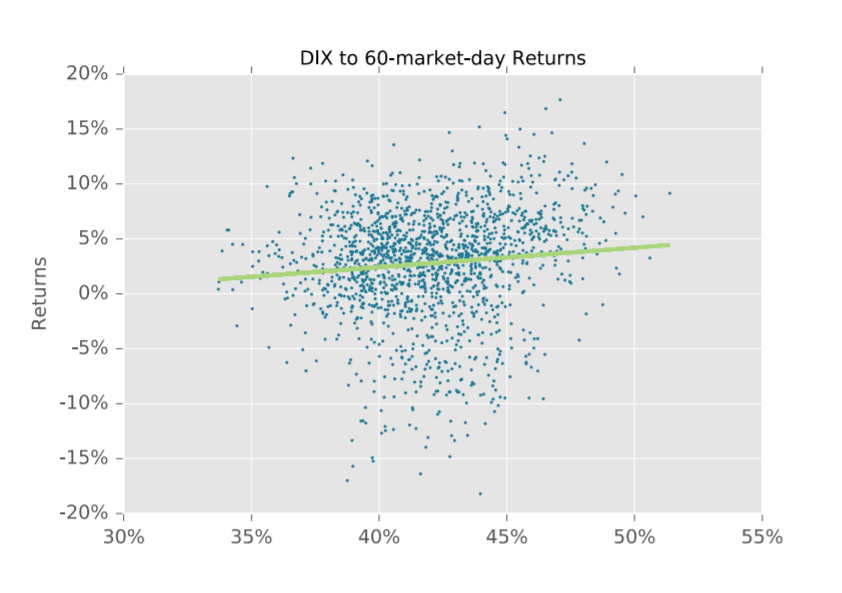
\includegraphics[width=\textwidth]{DIX to 60-market-day Returns.png}        
    %\caption{Caption}
    %\label{fig:my_label}
\end{figure}

\subsection{Data used for DIX}
\begin{itemize}
    \item The data used to test intraday short volume to stock returns is "FINRA's "Reg SHO Daily Files."
    \\ \url{http://regsho.finra.org/regsho-Index.html}
    \item Ignore "short-exempt" volume.
    \item FINRA's Monthly Short Sale Transaction Files (All off exchange short sale transactions with timestamps)
    \\\url{https://www.finra.org/filing-reporting/trf/trf-regulation-sho-2020}
    \item CBOE(formerly BATS) exchanges have made their short volume data available, NASDAQ and NYSE haven't.
    \\\url{https://markets.cboe.com/us/equities/market_statistics/short_sale/?mkt=bzx}
    \\\url{https://markets.cboe.com/us/equities/market_statistics/short_sale/?mkt=byx}
    \\\url{https://markets.cboe.com/us/equities/market_statistics/short_sale/?mkt=edga}
    \\\url{https://markets.cboe.com/us/equities/market_statistics/short_sale/?mkt=edgx}
    \item Lit exchanges will tend to have fewer large institutional cross trades and thus higher short volume. Taken together, they will add up to around SEC's aforementioned 49\% figure.
    
\end{itemize}

\newpage

\section{GEX}
\subsection{VIX}
\begin{itemize}
    \item The S\&P 500 Index (SPX) has a large and deeply liquid market for cash-settled options. 
    \item The CBOE Volatility Index (VIX) is derived from these options.
    \item VIX = 30-day option implied variance
    \item VIX uses a selection of quoted prices to derive what can be considered, put simply, an estimate of how much the S\&P500 will move int he future.
    \item VIX is effective at predicting 30-day future realized volatility - the CBOE places the correlation at 0.75. 
    \item VIX is more strongly correlated (0.85) to the realized volatility of the previous month. 
    \item VIX clearly fails to generate suitably distinguishable future stock return distributions at its lower readings.
    \item 1-day standard deviation of SPX returns following the lowest quartile of spot VIX closes (0.51\%) is not much different that the second-lowest quartile (0.66\%).
    \item A VIX of 12 means about the same as 15 when predicting variance.
    \item Comparing the highest and second-highest of GEX to subsequent SPX variance, the 1-day standard deviations are 0.55\% and 0.85\%. 
    \item Low VIX or high GEX predicts low volatility.
    \item The greater granularity of the GEX distributions suggests that there is some element of market volatility that is simply not able to be captured by the VIX model/any other variance metric based on quoted option prices.
    \item GEX focuses on quantity and characteristics of all existing option contracts at all strikes/expirations and the market participants who trade them
\end{itemize}

\begin{figure}
    \centering
    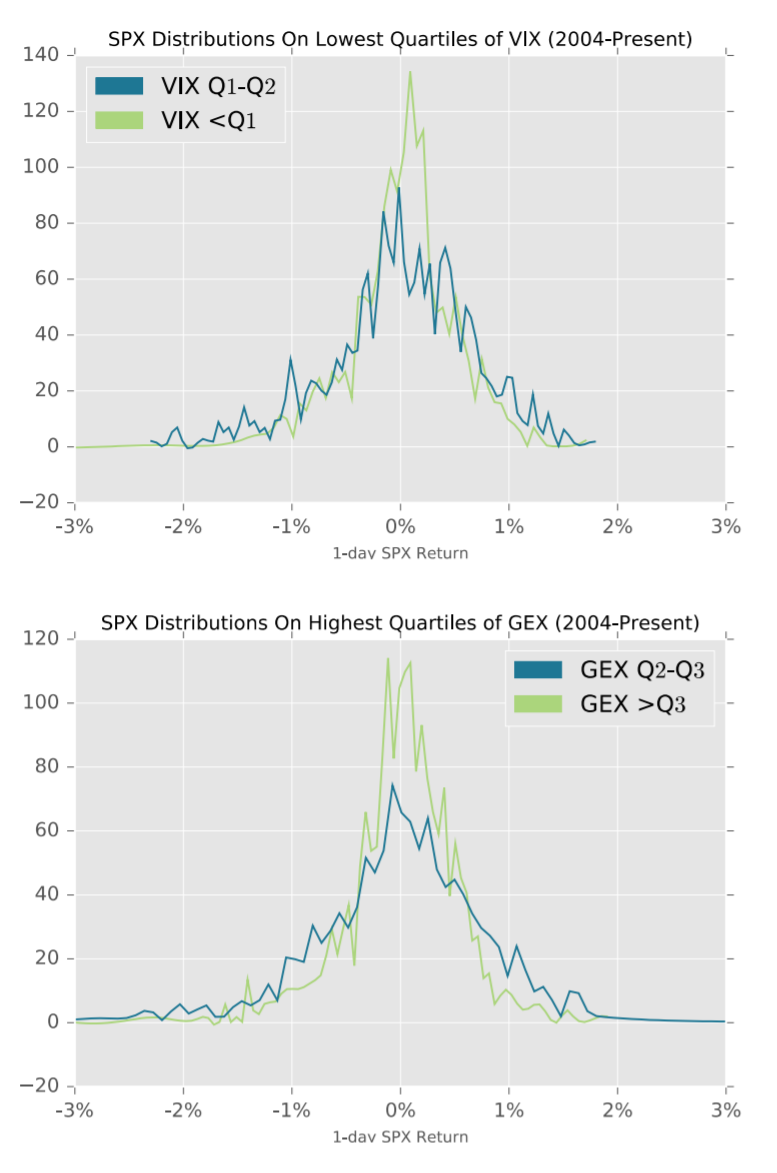
\includegraphics[width=\textwidth]{1-day SPX Return Vs. GEX_DIX.png}        
    %\caption{Caption}
    %\label{fig:my_label}
\end{figure}

\newpage


\subsection{Dynamic Hedging}
\begin{itemize}
    \item The predictive power of GEX is driven by the necessity of option dealer's(MMs) re-hedging activities.
    \item An option MM limits his exposure to deltas in order to limit risk and realize profit.
\end{itemize}

\subsubsection{Example}
\begin{itemize}
    \item If a MM sells a single 20-delta put contract then he must short-sell ~20 shares of the underlying stock in order to temporarily neutralize the convexity effect of the option's gains and losses. 
    \item Since the convexity itself cannot be hedged away, the MM must commit to re-hedging the option to its new delta whenever the underlying price changes enough to justify action.
    \item If the price of the underlying falls and the put delta rises from 20 to 50, the MM will be compelled to short-sell an additional shares of the underlying to stay delta-neutral. 
    \item If the put delta falls to 0, the market-maker would buy back the previously shorted shares. 
    \item Puts expire = buying of stock, puts gaining in value = selling of stock.
\end{itemize}

\subsection{Four Assumptions}
The size and liquidity of the option market is what makes it possible to glean predictive information from the impact of hedging activity. There are however, some assumptions. 
\begin{enumerate}
    \item All traded options are facilitated by delta-hedgers. 
    \begin{itemize}
        \item Every option contract is bought/sold by a market participant who's business is to profitably manage a book of options.
    \end{itemize}
    \item Call options are sold by investors; bought by market-makers. 
    \begin{itemize}
        \item It is difficult to determine the "direction" of a trade in an ultra-liquid market.
        \item It is apparent from an analysis of skew, open interest at strike, and (circularly) the effects of GEX, however, that the practice of call overwriting: selling covered call with higher strike than current underlying (and stock collaring: buy OTM put + sell OTM call) drives the market for calls.
    \end{itemize}
    \item Put options are bought by investors; sold by market-makers
    \begin{itemize}
        \item Used primary by investors who are already exposed to the underlying market.
        \item The "protective put" commands a premium for this reason, thus influencing the apparent vertical skew of index options
    \end{itemize}
    \item Market-makers hedge precisely to the option delta. 
    \begin{itemize}
        \item If MMs hedged their deltas every time an option's delta changed, they would be trading incessantly.
        \item In reality, MMs utilize "hedging bands" to balance the twin challenges of hedging costs and delta risk.
        \item Since it's not feasible to gauge the breadth of every MM's hedging band, we simply use the delta of the option.
    \end{itemize}
\end{enumerate}


\subsection{GEX Computation}
\begin{itemize}
    \item Gamma = first derivative of delta = rate of change of delta per 1-point move in the underlying.
    \item To calculate the GEX of an option, we need to determine the share impact of that potential change in delta on a MM's book.
\end{itemize}

\subsubsection{Example:}
\begin{itemize}
    \item If gamma of a single 50-delta call is 10, we can assume that a MM will re-hedge that option to either 40 or 60 delta in the event of any $\pm$ point move in the underlying.
    \item If underlying moves up 1 point: New delta = 60 and MM will short-sell 10 shares
    \item If underlying moves down 1 point: New delta = 40, market-maker will buy back 10 shares
\end{itemize}

\subsubsection{GEX Formula}

\begin{itemize}
    \item To calculate the GEX (in shares) of all call options at a particular strike:
    \begin{align}
        \text{GEX} = \Gamma \cdot \text{OI} \cdot 100
    \end{align}
    \item In case of put options where MM is short a put call:
    \begin{align}
        \text{GEX} = \Gamma \cdot \text{OI} \cdot (-100)
    \end{align}
    \item The GEX of a stock is the summation of GEX at every strike price in every available contract
\end{itemize}
   
\subsection{Market Impact}
\begin{itemize}
    \item Positive GEX(MMs short lots of calls) implied that option market-makers will hedge their positions in a fashion that stifles volatility (Buying into lows: buy back shares when delta decreases on long calls to stay delta neutral, selling into highs: short more shares when delta increases).
    \item Negative GEX implies the opposite (Selling into lows, buying into highs) thus magnifying market volatility.
    \item Corollary: GEX figure approaching zero will allow the market to move naturally and without any particular interference from MMs re-hedging activities. 
\end{itemize}

\begin{figure}[!ht]
    \centering
    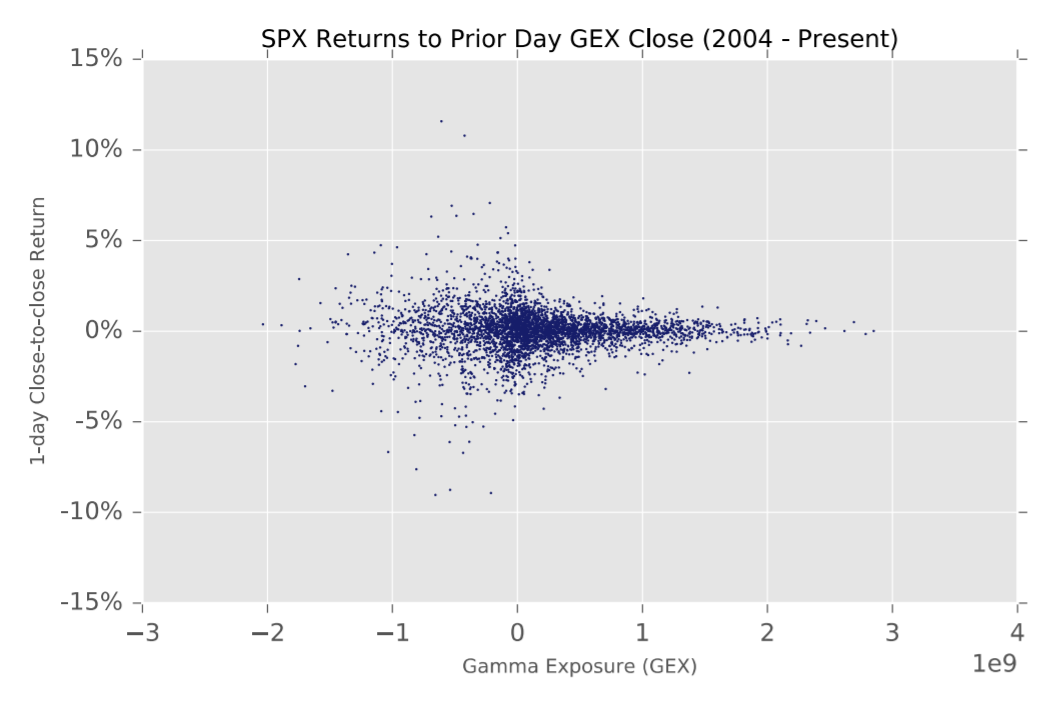
\includegraphics[width=\textwidth]{SPX Returns to Prior Day GEX Close.png}        
    \caption{Note the exponential increase in volatility as GEX trends below zero, and the gradual tightening of the distribution as GEX rises.}
    %\label{fig:my_label}
\end{figure}

\newpage
\subsection{The Implied Order Book: Measuring S\&P 500 Liquidity with SPX Options}
The stock market is a ledger of who is willing to buy/sell at what price (A limit order book). It shows where there is supply and demand. Because of the competitive nature of the market, most of the liquidity that is visible is in one way or another, a bluff. 
\begin{itemize}
    \item 
\end{itemize}

\end{document}
